\documentclass{beamer}
\usepackage[ngerman]{babel}
\usepackage[T1]{fontenc}
\usepackage[utf8]{inputenc}

\title{Privacy Preserving Record Linkage on Flink}

\subtitle{Big Data Praktikum}

\author{T. Hornoff \and M. Franke}

\institute{Universität Leipzig \\ Abteilung Datenbanken}

\date{04.08.2016}

\AtBeginSection[]
{
  \begin{frame}
    \frametitle{Inhalt}
    \tableofcontents[currentsection]
  \end{frame}
}

\begin{document}

	\frame{\titlepage}

	% ------------- Einleitung -------------- %
	\section[Section]{Einleitung}
    
    \begin{frame}
    		\frametitle{PPRL}
         Something about PPRL.
         
         \begin{itemize}
         		\item Auffinden von gemeinsam genutzten Datenelementen (Korrespondenzen)
         		\item Verbindung von Datensätzen aus einer oder mehreren Datenquellen
         		\item Herausforderungen
                \begin{itemize}
                    \item Schutz personenbezogener Daten
                    \item Sicherung der Privatspähre, des Datenschutzes \& der Vertrauchlichkeit
                    \item Wachsende Datenmengen (Skalierbarkeit)
                    \item Qualität der Daten
                \end{itemize}
         		\item Zahlreiche Anwendungsgebiete
                \begin{itemize}
                    \item Gesundheitsfürsorge
                    \item Betrugserkennung
                    \item Finanzinstitutionen \& Banken
                    \item Unternehmensanwendungen
                \end{itemize}
         \end{itemize}
    \end{frame}
    
    \begin{frame}
    		\frametitle{Flink}
        	Something about Flink.
    \end{frame}

	\begin{frame}
    		\frametitle{Bloom Filter}
            \begin{figure}[H]
                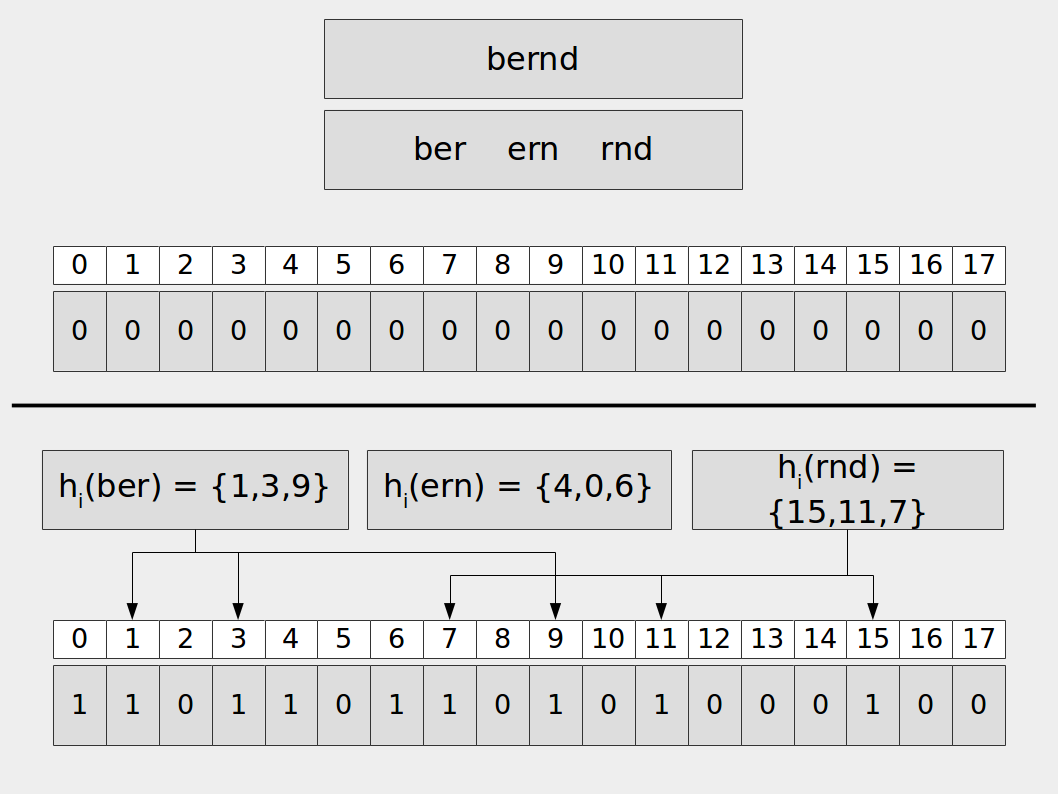
\includegraphics[width=\textwidth]{bloom_qgram.png}
            \end{figure}
    \end{frame}
    
    \begin{frame}
        \frametitle{Locality Sensitive Hashing (LSH)}
            Locality Sensitive Hashing
            \begin{itemize}
                \item Jaccarrd-Similarity
                    \begin{itemize}
                        \item jaccard\ldots
                    \end{itemize}
                \item Hamming-Distance
                    \begin{itemize}
                        \item hamming\ldots
                    \end{itemize}
            \end{itemize}
    \end{frame}
   % -------------------------------------------- %
   % ------------- Realisierung ----------- %
    \section[Section]{Realisierung}
    \begin{frame}
    		\frametitle{Ablauf}
    		Datensatz,
         Ablauf unseres PPRL-Prozesses,
         Arten der Parallelisierung (Record/Token-Ebene),
         Laufzeitverhatlten,
         Transferierte Daten,
         ...
    \end{frame}
    
\end{document}
